\subsection{(\S3) Understanding Consciousness Through the Theory of Psychological Types}

\begin{itemize}

\item When Jung began to work on the psychological problem that he was
attempting to solve with his theory of types, he had an international
reputation as an investigator of the unconscious.

\item This perception, which I would call a prejudice, has affected the
reception of the subject of psychological type among depth psychologists ever
since, including the majority of analytical psychologists working today.

\item The type theory was a contribution to the problem of the standpoint from
which the individual experiences the unconscious. That the conscious standpoint
of the patient could hardly be ignored Jung had already learned from his
practical experience as a psychiatrist attempting to understand dreams and
symptoms, for the patient's conscious stance often turned out to be what the
unconscious was actually responding to.

\item So etymology indicates that the phenomena of consciousness and conscience
are somehow related and that the experience of consciousness is made up of two
factors -- `knowing' and `withness'. In other words, consciousness is the
experience of knowing together with an other, that is, in a setting of twoness.
-- Edinger, 1984, \P 36

\item By the time Jung set out to write Psychological Types, consciousness had
come to mean for him the way the reality of the psyche is both accessed and
assessed, or what he sometimes called ``understanding'' (Jung, 1914/1972),
which he made the basis of his entire approach to psychology. Consciousness, in
this sense, was the indispensable investigative tool for all further work on
the unconscious.

\end{itemize}

\subsubsection{The individuation of consciousness}

\begin{itemize}

\item What is not immediately apparent to those who try to approach Jung's
psychology as if it were another science, albeit a science of the unconscious,
is that consciousness, for Jung the tool with which the unconscious must be
investigated, is an emergent property of the unconscious itself (Camberay,
2006).

\item There he defines consciousness in terms of its relation to the ego:
\begin{quote}
By consciousness I understand the relatedness of psychic contents to the ego...
in so far as they are sensed as such by the ego. In so far as relations are not
sensed as such by the ego, they are unconscious. Consciousness is the function
or activity which maintains the relation of psychic contents with the ego.
Consciousness is not identical with psyche, since, in my view, psyche
represents the totality of all the psychic contents, and these are not
necessarily all bound up directly with the ego, i.e. related to it in such a
way that they take on the quality of consciousness. There exist a great many
psychic complexes and these are not all, necessarily, connected with the ego.
-- Jung, 1921/1923, pp. 535-536
\end{quote}

\item Jung's own way of speaking about the growth of consciousness in human
beings tended to be simpler, and from a contemporary standpoint, more soulful.
For instance, while giving a seminar, he was once asked, ``Is not individuation,
in our sense of the word here, rather living life consciously? A plant individuates
but it lives unconsciously.'' Jung's answer was:
\begin{quote}
That is our form of individuation. A plant that is meant to produce a flower is
not individuated if it does not produce a flower, it must fulfill the cycle;
and the man who does not develop consciousness is not individuated, because
consciousness is his flower; it is his life, it belongs to our process of
individuation that we shall become conscious. -- Jung, 1934/1997, pp. 758-759
\end{quote}

\item Sticking to Jung's metaphor of flowering, I find it best to say that if a
person individuates, that is, goes on to flower, then the various functions of
consciousness that Jung describes in Psychological Types will be the petals of
his or her flower. (This notion does not assume that consciousness originates
in the ego)

\item The idea that consciousness already resides in some form in the
unconscious gives another meaning to the idea of `knowing together with an
other.' The idea of a teamwork between ego-consciousness and a consciousness
that already resides in the unconscious is particularly appropriate to the
understanding of the psychological functions Jung has called `thinking,'
`feeling,' `sensation,' and `intuition.' In Psychological Types, he conceives
these as two pairs of opposites: thinking and feeling (evaluative functions)
defining one axis of consciousness, sensation and intuition (perceptive
functions) the other. Asked for definitions of these four functions of
consciousness, Jung told an interviewer:

\begin{quote}

there is quite a simple explanation of those terms, and it shows at the same
time how I arrived at such a typology. Sensation tells you that there is
something. Thinking, roughly speaking, tells you what it is. Feeling tells you
whether it is agreeable or not, to be accepted or rejected. And intuition --
now there is a difficulty. You don't know, ordinarily, how intuition works.
When a man has a hunch, you can't tell exactly how he got at that hunch, or
where that hunch comes from. There is something funny about intuition. [Jung
gives an example.] So my definition is that intuition is a perception via the
unconscious. -- Jung, 1957/1977, p. 306

\end{quote}

\item I like to read that amplification of the intuitive function as a gloss on
the purpose that all the functions of consciousness -- thinking, feeling, and
sensation too -- serve. All of them are required because life itself presents
problems that are already differentiated in such a way that only a particular
function of consciousness can solve them. In that case, we would be justified
to speak of a problem presented by a patient as a thinking problem a feeling
problem, an intuitive problem, or a sensation problem. Similarly, a dream,
which reveals to us ``the actual situation in the unconscious'' (Jung,
1948/1960, \P 505) of a client, lays out the situation for us in such a way
that we can `type' it, if we wish, as a thinking situation, a feeling
situation, an intuitive situation, or a sensation situation. The problem is
then coming up with the function of consciousness appropriate to the situation,
or, in other words, meeting the situation's own peculiar consciousness as to
what it is with a consciousness that matches it. From this perspective, the
development of consciousness involves the ability to summon the various
functions at appropriate times in appropriate ways.

\item This function is the area of our consciousness that is least under the
control of our good intentions, slowest to take training despite our best
efforts, and most tied up with the unconscious. Hillman's description of the
inferior feeling function well conveys the problem that arises on the basis of
this association with what is ordinarily repressed:

\begin{quote}

Inferior feeling, to sum it up, may be characterized by contamination with the
repressed which tends to manifest, as the Scholastic would have said, in ira
and cupiditas [anger and desire]. Inferior feeling is loaded with anger and
rage and ambition and aggression as well as with greed and desire. Here we find
ourselves with huge claims for love, with massive needs for recognition, and
discover our feeling connection to life to be one vast expectation composed of
thousands of tiny, angry resentments. This expectation has been called an
onmipotence fantasy, the expression of the abandoned child with his leftover
feelings that nobody wants to take care of -- but is this enough? Omnipotence
is more than a content; rather it expresses, as does the child, an impoverished
functioning that insists upon more sway and exercise. Without this exercise,
feeling turns upon itself, morbidly; we are envious, jealous, depressed,
feeding our needs and their immediate gratification, then rushing out
intermittently to meet someone to help or for help. \ul{The cat neglected
becomes the unconscious tiger.} \flushright -- Hillman in von Franz \& Hillman,
1971/1998, p. 135

\end{quote}

It should be pointed out that this description of the emotional attitude of a
function of consciousness in the inferior position is strikingly similar to
Adler's description of the inferiority complex (Ellenberger, 1970, pp.
612-613).

\item For his seminars, Jung liked to diagram this hierarchy in various ways
according to a fourfold model, specifying a superior function, an auxiliary
function, a tertiary function, and an inferior function. I have standardized
Jung's diagram as follows for my own classes on psychological types:
(Figure~\ref{fig:beebe-figure-31})

\begin{figure}[h!]
  \centering
  \begin{tikzpicture}[font=\small\rmfamily,every node/.style={text=black}]
    \node[anchor=east] (aux) at (-2, 0) {Auxiliary function};
    \node[anchor=west] (ter) at (2, 0) {Tertiary function};
    \node[anchor=south] (sup) at (0, 2) {Superior function};
    \node[anchor=north] (inf) at (0, -2) {Inferior function};
    \draw[black, thick] (aux.east) -- (ter.west);
    \draw[black, thick] (sup.south) -- (inf.north);
  \end{tikzpicture}
\caption{Jung’s hierarchy of the types of consciousness in an individual}
\label{fig:beebe-figure-31}
\end{figure}

This diagram can be read as a stick-figure representation of a right-handed
person, who might be imagined standing erect with feet together and back placed
flush against a blackboard with his or her arms spread-eagled, for the purpose
of revealing the relations of his or her functions of consciousness. Each of
the qualifying adjectives for the four functions shown in the diagram --
superior, auxiliary, tertiary, and inferior -- describes the `position' of one
of the person's four functions of consciousness in relation to the others. What
is suggested is a hierarchy of the functions that, though it begins according
to their degree of differentiation, ends up being as qualitative as it is
quantitative. That is to say, the way the function is experienced, both by the
person who possesses it and by the others he or she deals with, is as much a
result of its position in the total hierarchy of functions as of its actual
degree of differentiation. The positions themselves convey certain qualities to
the functions that occupy them, as von Franz and Hillman demonstrated for the
`inferior' function and I have proceeded to do for the other three positions.

Further, these named positions, as Figure~\ref{fig:beebe-figure-31} shows,
define a pair of axes, a vertical axis (between the superior function and
inferior function), which I think of as the `spine' of consciousness defining
the person's conscious standpoint, and a horizontal axis (between the auxiliary
and tertiary functions), which for me are the `arms' of consciousness, since it
is the task of these functions to handle the relation to the world once the
individual standpoint of the person is established.

\end{itemize}

\subsubsection{Type as a method of analysis}

\begin{itemize}

\item My father, a military man who had commanded a battalion in Korea, was an
extraverted thinking type. When I would interrupt the nightly radio news
broadcast to offer opinions of my own about what the developments might
signify, my father would say, ``Shut up, son. You don't learn from people who
know nothing.'' My analyst, also a man, never interrupted, or almost never.

\item ... in accord with the then prevalent Jungian notion that feeling was
more feminine than thinking.

\item No such impediment to empowering my thinking came up in my analyst's
initial overt countertransference, and so I experienced the ideal conditions
for a therapy described by Carl Rogers and his colleagues: genuineness,
unconditional positive regard, and accurate empathic understanding (Rogers \&
Truax, 1967). For this reason, I became precociously clear about the nature of
my own typology as part of my self-experience. I believe that only some such
direct experience of the types as one's own, and the permission to consider
them in one's own way, can enable a patient to avail himself or herself of the
individuation potential of the type theory. Otherwise, type becomes another way
to learn from others what one is, and a new set of tasks to be learned in the
effort to adapt more effectively to the environment. There can be value in type
still in discovering new energy for adaptation, but this is not the same as
individuation.

\item As I have indicated in other writings (Beebe, 1988, 1992), I believe that
it is only through experiencing one's personal, `little-s' self in a way that
has `integrity in depth' that the `big-S' Self of Jungian psychology, the
instinctive knowledge of how to live, can be authentically accessed.

\item The opening up of my typology led to a great deal of energy pouring into
my psyche from the Self. My new problem, replacing the depression I had come to
therapy with, was a tendency to get too excited. I sometimes imagined my
superior intuition was like the head of a rocket ship, ready to take
off.\footnote{John Beebe is ENTP type.} I needed desperately to hold myself to
the earth, to stay with the tasks associated with medical training. At that
early stage, my inferior function, sensation, simply did not have the necessary
weight, the specific gravity, to anchor me. But I noticed that my auxiliary and
tertiary functions could be enlisted to keep me connected to the demands of the
world. Thinking, after intuition my strongest function, and therefore my
auxiliary, helped me to define my situation and identify the issues I needed to
work on.  And my feeling, less confident and more vulnerable, kept me guessing
what my impact was on other people and working to discover what my actual
relationships with them were. The combined effect of using these two processes,
thinking and feeling, was to slow me down and keep me out of the most
irrational flights of my intuition. I first became aware in an inner way that
my thinking and feeling form an axis, just as my superior intuition and
inferior sensation do, when I had the following dream: A father (a man who was
maybe in his fifties) was chasing his son (a young man in his twenties) around
a dining room table, waving a butcher knife.

\item Working on this dream in my analysis, I was able to associate to the
image of the young man. Although the echoes of my feeling reactions to a
critical father were clear, the young man in my dream, in his fearfulness, was
not anything like my waking personality. At that time, if anything, I had not
learned to fear.

\item The son in the dream reminded me of a young man I know at the time, whose
feeling function was well developed and who thought very slowly. The butcher
knife, with its capacity to cleave and dissect, seemed to me the image of a
thinking function that makes separating distinctions between things.  That an
older man wielded it in a terrorizing way toward a younger suggested to me,
when I thought about it intrapsychically, that a more developed function was
somehow bullying a less developed one. The dream may, of course, have been a
commentary on the way I used thinking around my feeling-type friend, but at the
time I also needed to focus on how I was relating to myself. I decided that the
father symbolized my auxiliary thinking and the son my tertiary feeling.  They
are related to each other --- in the same family -- but in my situation at that
time the relationship appeared to be a sadomasochistic one.

\item It did not satisfy me to see the dream merely as a reenactment of the
humiliations I had received from my father in childhood, such as when I had
tried, rather rudely, to express the thoughts that occurred to me at the dinner
table while his `news briefing' was on the radio. Yes, my father had bullied my
introverted thinking with his extraverted thinking, but what I was doing to
myself now, as reflected in the dream, was allowing my relatively strong
thinking function to browbeat my much less developed feeling function.

\item Chastened by the dream, I gradually became less aggressive about applying
overriding thinking formulations to the understanding and dismissal of my
feeling when it was upset. In time, my thinking became less tyrannical and
began to take a more protective attitude toward my shakier, immature feeling.
My relation to feeling-type patients and friends also got kinder.

\item Dr. Detloff, however, was quite clear that introverted sensation and
extraverted sensation were so different that he wondered why they were even
both called `sensation.' Later I came to see that introverted sensation
concerns itself primarily with finding order, organizing experience, and
monitoring the comfort of the body on the inside, whereas extraverted sensation
involves compelling, often shared, experiences of the textures, smells, sights,
sounds, and tastes of the world --- a direct relationship with reality.
Similarly, I decided that introverted feeling is mainly concerned with the
values that matter most to oneself, while extraverted feeling seeks to connect
with the feelings of others. Extraverted intuition, as friends often verified
after some of my uncannily telepathic moments in their presence, seemed rather
easily to pick up on what was going on in other people's minds, and it was
certainly seeing possibilities in what was more consciously shared with me that
others might never have imagined; whereas introverted intuition, I noticed (for
instance, in Jung) looked at the big picture in the unconscious, where the
gestalts that moved nations, religions, and epochs lay, even in the midst of
apparently `individual' experience. And the two kinds of thinking, though both
concerned with defining things, also did so in very different ways: extraverted
thinking such as my father's was interested in definitions that would hold true
for everyone, according to ideas everyone might agree with, whereas introverted
thinking such as mine had to reflect on whether a particular construction
really accorded with the conviction of inner truth, regardless of what the
received opinion might be.

\item Then I dreamed of a women sitting alone in a room. She was Chinese and
had a glum look on her face. The room she was in was bare, without other
furniture than the chair she was stting in. This was so because her husband
spent all his money doping and gambling and so had nothing to bring home. My
analyst was very insistent about the importance of this dream. ``She doesn't
have anything,'' she pointed out.

\item I associated to the woman. I knew her in life: she was the laundress at
the Chinese launderette to which I entrusted my washables at that time. A
practical, unadorned woman, she worked very efficiently. She was clearly no
extravert, but she was quite concerned with sensation matters in her
introverted way.  I decided she was an introverted sensation type. I had
recently read von Franz's essay on the inferior function and also Gareth Hill's
essay on ``Men, the anima and the feminine'' (1998), which at that time was
unpublished, but described eight types of anima, using both the four function
types (feeling, thinking, intuition, and sensation) and the two attitude types
(introverted and extraverted) to arrive at his eight possibilities for the type
of the anima, just as von Franz had done in establishing eight types of
inferior function in her essay.

\item The husband in the dream who was given to gambling seemed to me to
represent a less flattering side of my superior function, extraverted
intuition. That seemed to fit the image of the husband as a gambler, someone
who pursues possibilities and takes his energy into the world, leaving his
introverted wife at home alone, not giving her much. But what did this have to
do with me? I did not drink and gamble, but I was drawn to chase after
possibilities to extend my life, even after it was time to go home and rest.
The newest movie, the latest book, even the next dream one of my patients would
bring to me, were causing me to transgress the limits of my personal comfort.
For the first time, the importance of the extravert/introvert distinction
really was brought home to me. If the husband represented my unbalanced
extraversion, the clear message of the dream was that I was neglecting the
introverted side of myself, represented by the forlorn and unfurnished anima
figure, the Chinese laundress. The dream was saying, very specifically, that my
introverted sensation was not getting anything from me. When I conveyed this
conclusion to my analyst, she said, ``I couldn't agree more.''

\item I thought long and hard about how to rectify that state of affairs.
Introverted sensation, I knew by this time, lives on the inside of the body,
and seeks to keep it from getting overstimulated, overheated, too tired, too
hungry, or too filled with the wrong foods, etc. I looked at what was happening
with my patients in my developing psychotherapy practice. I was very excited to
hear everything they were telling me, so much so that I was listening with
bated breath, neglecting even to breath properly. No wonder I came home to
migraine headaches: I was retaining carbon dioxide. I made up my mind that I
would have to attend to my breathing while listeninig to patients. This opened
a series of spaces that alloed me to be aware of my body as I practiced
therapy. I then noticed that in my body, as I attended to it, were clues to
what was going on in my patient beyond anything dream interpretation could have
revealed. If my stomach or chest felt tense, that was a signal that my patient
was feeling `uptight.' I found if I attended to these sensations, and
eventually took up with the patient the feelings I was introjectively
identifying, relevant material would emerge which would move the therapy
forward. When I succeeded in getting the patient to express the feelings that
my body had picked up, I wouldn't leave the session with a headache, and I
would end the day of doing psychoterapy energized, not depleted. Apparently
this method was a tonic for my inner life. A subsequent dream about the Chinese
laundress found her happier: her husband had been taking her out for ice cream!

\item There is a tradition in Jungian analysis that the type problem becomes
especially important when the inferior function starts to `come up' as a topic
in analysis, and that then one needs to pay very close attention to the type.
Certainly that turned out to be true in my case. Once I knew that my anima was
an introverted sensation type, and that I tended not just to be woefully
inefficient in this area (as I had recognized as soon as I realized I was an
intuitive) but also destructively neglectful (which I had not realized until I
dreamed of the Chinese laundress whose husband was not providing for her), I
became much more interested in the exact situation of all my functions, and
gave a lot of thought to what in me was exraverted and what introverted.

\item There is something seductive about the sense of wholeness that comes with
the number four, which Jung consideres the archetypal number designating the
`big-S' Self. I was at least seven years into my analysis before the four
functions that make up my typology were clear to me, and it was hard not to
believe that I had somehow `arrived,' from the standpoint of individuation,
even though I was only thirty-four years old. Today this seems to be a bit like
the naivety of a relatively young person, but the inflation of self-discovery
can threaten at any age. To assume that type development ends with the
discovery of the inferior function, at which point the Self is constellated and
from then on one is engaged in relating to the unconscious in its deeper
aspect, can actually interfere with the development of consciousness.  In
reality, type remains an issue throughout the individuation process, although
analysts do not always recognize this.

\end{itemize}

\subsubsection{Type development}

\begin{itemize}

\item Elizabeth Murphy also takes up this theme in her book The Developing
Child (1992, pp. 12–13), in which she points out that the superior and
auxiliary functions may develop naturally in childhood, but that the tertiary
and inferior functions normally do not appear until adulthood. I believe that
my first analysis unblocked this normal developmental process in me. One of
Myers’s most important ideas, which she and her mother had culled from Jung,
was that “For all the types appearing in practice, the principle holds good
that besides the conscious main function there is also a relatively
unconscious, auxiliary function which is in every respect different from the
nature of the main function” (Jung, 1921/1923, p. 515, quoted in Myers, 1980,
p. 19).

As Myers insisted:
\begin{quote}
The operative words are “in every respect.” If the auxiliary process differs
from the dominant process in every respect, it cannot be introverted where the
dominant process is introverted. It has to be extraverted if the dominant
process is introverted, and introverted if the dominant process is extraverted.
--- Myers, 1980, p. 19
\end{quote}

\item What I find most striking in these passages is Jung’s assumption that
only one function, the superior, is likely to be particularly differentiated.
Therefore, the other functions all take on the unconscious character of the
inferior function, and operate in a crudely compensatory way. That actually
describes the undifferentiated way my unconscious compensated me before I went
into analysis, but it was not particularly helpful to understanding the ways my
function types sorted themselves out, as to attitude, once they started to
become differentiated in analysis.

\item One way I was experiencing this differentiation was that I was becoming
more particular, and not less, when I practiced psychotherapy, so that I often
suffered if a person in my practice had introverted feeling that I could not
take care of with my extraverted feeling. I devoted a lot of attention to this
problem, and was particularly helped by a passage in von Franz’s essay on the
inferior function in Lectures on Jung’s Typology. She had been asked the
question, “Does an introverted feeling type experience introverted thinking, or
is it always extraverted thinking?” She replied:
\begin{quote}
If you are an introverted feeling type, you can also think introvertedly. You
can naturally have all the functions all ways, but it won’t be such a great
problem, and there will not be much intensity of life in it. Jung has said that
the hardest thing to understand is not your opposite type—if you have
introverted feeling it is very difficult to understand an extraverted thinking
type—but the same functional type with the other attitude! It would be most
difficult for an introverted feeling type to understand an extraverted feeling
type. There one feels that one does not know how the wheels go round in that
person’s head; one cannot feel one’s way into it. Such people remain to a great
extent a puzzle and are very difficult to understand spontaneously. Here the
theory of types is tremendously important practically, for it is the only thing
which can prevent one from completely misunderstanding certain people.
--- von Franz \& Hillman, 1971/1998, p. 64
\end{quote}

\item I addressed the subject of type incompatibility in my first full-length
essay on the role types play in transference, countertransference, and the
therapeutic interaction (Beebe, 1984). In that publication, I recommended that
analysts try to determine for each of a client’s four functions whether that
function is being used in an introverted or an extraverted way. I also
suggested that the analyst should make an effort to figure out if he or she is
deploying that function with the same, or with an opposite, attitude with
respect to introversion and extraversion. It is on this basis, rather than
whether one person in the therapeutic dyad has feeling as the superior function
and the other thinking, or has an extraverted superior function when the other
has an introverted superior function, that I established type compatibility,
meaning whether there would be easy empathic understanding between the partners
or whether there would be frequent clashes.

\item That, for Jung, is whether the person’s superior function is rational
(his term for the evaluative functions, thinking and feeling) or irrational
(his term for the perceptive functions, sensation and intuition).

\item For me, Jung’s approach is the more psychological. When assessing type
compatibility between people, I prefer to look at each individual’s vertical
axis, or spine of consciousness, which connects the superior and inferior
function, rather than privileging extraversion.

\item Von Franz (1970) and Henderson (1967), focusing on its role in masculine
development, relate the excessive reliance on this archetype in daily
interactions with others to the narcissistic mother complex of the immature
man.

\item I am using this term, in tandem with puella aeterna, Latin for ‘eternal
girl,’ to refer to the eternal youth in all of us, the brilliant but volatile
side of ourselves that is by turns the seemingly immortal Prince or Princess
and the helplessly vulnerable, wounded boy or girl.

\item The inferior function is the door through which all the figures of the
unconscious come into consciousness. Our conscious realm is like a room with
four doors, and it is the fourth door by which the shadow, the animus or the
anima, and the personification of the Self come in. -- William Alex

\item She later adds that “when one has become somewhat conscious of the
shadow, the inferior function will give the animus or the anima figure a
special quality” so that, if personified by a human being, the anima or animus
will “very often appear as a person of the opposite function” (von Franz \&
Hillman, 1971/1998, pp. 67–68).

\item In my own work on myself and with patients, I most often found the
inferior function, with its uncanny emotionality, to have the character of the
anima or animus,7 the ‘other’ within us, which becomes profoundly upset when
its ideals are not met and nearly ecstatic when they are. It had been
symbolized that way by my dreams of the Chinese laundress. I could then diagram
my four functions again, showing the archetypes associated with them as I had
encountered them.

\item My shift into Latin in naming the archetypes associated with the tertiary
and inferior functions is deliberate. These functions, though still part of
one’s complement of ego-syntonic consciousnesses, are more archaic than the
superior and auxiliary and present themselves in more classically ‘archetypal’
ways, having a god-like entitled quality to them, whereas the superior and
auxiliary functions are more adapted to this time and place and more
considerate of the perspectives of one’s contemporaries.

\item \ovalbox{\it Beebe's model of type} This archetypal analysis of the first
four functions provided the basis for the model of type I was able to present
at the Chiron Conference for Jungian psychotherapists held at Ghost Ranch in
Abiquiu, New Mexico in 1983, and to write up in my 1984 essay, “Psychological
Types in Transference, Countertransference, and the Therapeutic Interaction.”
It has proved very helpful both to me and to others in clarifying how a
well-differentiated consciousness might arrange itself in the course of
individuation. We might note several features of this model.

\begin{figure}[h]
  \centering
  % Set font style and size for the nodes
  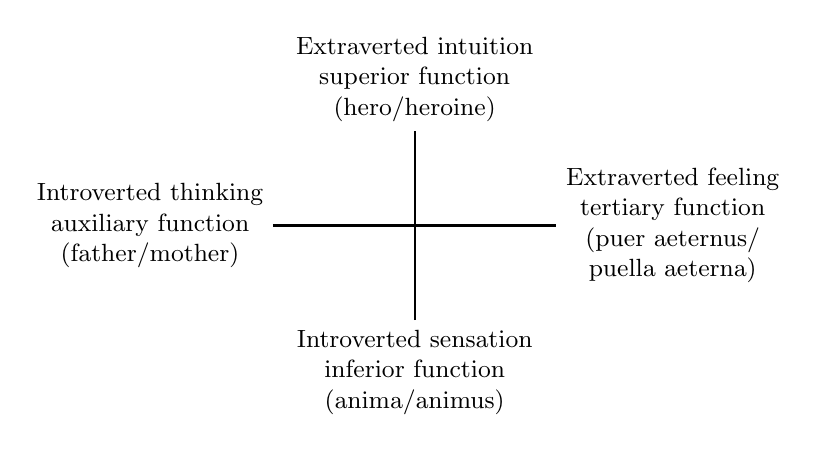
\begin{tikzpicture}[
    node_format/.style={align=center, font=\small},
    ]
    
    % --- Draw the Cross (Axes) ---
    % Horizontal line
    \draw[thick] (-1.8,0) -- (1.8,0);
    % Vertical line
    \draw[thick] (0,-1.2) -- (0,1.2);

    % --- Place Text Nodes ---
    
    % Top Function: Extraverted Intuition (Superior)
    \node[node_format, anchor=south] at (0,1.2) {
      Extraverted intuition \\
      superior function \\
      (hero/heroine)
    };

    % Bottom Function: Introverted Sensation (Inferior)
    \node[node_format, anchor=north] at (0,-1.2) {
      Introverted sensation \\
      inferior function \\
      (anima/animus)
    };

    % Left Function: Introverted Thinking (Auxiliary)
    \node[node_format, anchor=east] at (-1.8,0) {
      Introverted thinking \\
      auxiliary function \\
      (father/mother)
    };

    % Right Function: Extraverted Feeling (Tertiary)
    \node[node_format, anchor=west] at (1.8,0) {
      Extraverted feeling \\
      tertiary function \\
      (puer aeternus/ \\
      puella aeterna)
    };

  \end{tikzpicture}
  % The caption text, including the hyperlink for "FIGURE 3.3"
  \caption{FIGURE 3.3: My orientation with archetypal complexes}
  \label{fig:jungian_functions}
\end{figure}

\begin{enumerate}[nosep]

\item The model asserts, with Jung and subsequent Jungians, that if the
superior function is irrational the auxiliary will be rational, and vice versa.

\item It agrees with Myers and the MBTI counselors that if the superior
function is introverted the auxiliary will be extraverted and vice versa.

\item The model specifies the tertiary function as opposite in attitude to the
auxiliary just as the inferior is opposite in attitude to the superior.

\item Following the Jungian tradition, the model maintains that if the superior
function is rational, the inferior will likewise be rational; if the superior
function is irrational, the inferior function will also be irrational.

\item The tertiary function is represented as matching the auxiliary with
respect to rationality or irrationality.

\item The model therefore defines two axes of consciousness, one between the
superior and inferior functions (spine), the other between the auxiliary and
tertiary functions (arms). If the spine is rational, the arms will be
irrational and vice versa (see Figure 3.4).

\end{enumerate}

\item \ovalbox{\it type development and this model} I believe that this model
makes sense of the way the types differentiate in someone who is showing what
Myers calls “good type development” and Jung would call individuating according
to the law of his or her own being. It does not account for the many
falsifications of type (Benziger, 1995) that involve substituting other
functions out of a need to satisfy or defend against the type demands of an
environment that is not facilitative of individuation.

\end{itemize}

\subsubsection{Types of the shadow}

\begin{enumerate}

    \item \ovalbox{\it the four shadow functions has to be developed as well}
        Watsky pointed out that Jung lists eight functions of consciousness in
        Psychological Types. If someone succeeds in differentiating four of
        those functions to achieve the good type development of which Isabel
        Briggs Myers had spoken, Watsky said, it’s as if the north 40 acres of
        their psychological field has been hoed; the person still needs to
        cultivate the other four functions: the south 40. These four were
        presumably in shadow.

    \item \ovalbox{\it witch/senex} Like all the shadow archetypes, the witch
        'fights dirty' to defend the personality. She uses her capacity to cast
        spells that immobilize in an underhanded way, but this is a survival
        consciousness that resides in the shadow that can be used to stop
        others in their tracks when they are threatening the personality or its
        values. In terms of gender politics, the witch uses her feminine
        authority in a way that can be extremely paralyzing to the anima of a
        man. In a man’s psyche, the shadow side of the good father would be the
        senex, which exerts the same sinister limit-setting control when he
        ‘pulls rank,’ and which can similarly paralyze a woman’s animus. I have
        since learned that the negative ‘witch’ and the senex can appear in
        both genders as a kind of “withering authority” (Frey, 2011) that can
        be both dogmatic and mean. And I have often come to see the wisdom in
        the limit-setting of these archetypes, despite their initially sinister
        presentations.

    \item \ovalbox{\it shadow archetype carries opposite attitude} It was clear
        that the shadow archetype carries the same function of consciousness as
        its ego-syntonic counterpart, but with the opposite attitude with
        respect to extraversion and introversion.

    \item \ovalbox{\it opposing} The most unexpected discovery was the archetype I
        call the opposing personality, which is characterized by behaviors that
        may be described in the language of character pathology: oppositional,
        paranoid, passive-aggressive, and avoidant. This is a shadow that is
        very hard to see in oneself (it seems to fall in the blind spot of the
        superior function) and very easy to project onto another person,
        especially a person of the opposite sex. The archetype of the opposing
        personality often appears in dreams as a contrasexual figure, but,
        unlike the anima, the opposing personality is antagonistic to the ego
        rather than helpful in connecting it to the needs of the Self.
        Classical Jungians have sometimes identified this figure that opposes,
        criticizes, and seduces the ego as the ‘negative’ animus or anima, but
        this intuitive shorthand ignores the real type difference between the
        opposing personality and the anima or animus.

    \item \ovalbox{\it types should be used for sorting out the empirical
        material} In associating to a dream figure, it is important to try to
        establish the figure’s psychological type, which is often surprisingly
        easy to determine. At the Ghost Ranch conference, I called attention to
        Jung’s foreword to the Argentine edition of Psychological Types
        (1936/1971, p.  xiv) in which he had emphasized that the theory of
        psychological types should be used not as a way of classifying people
        but for “sorting out the empirical material” that comes up in the
        course of a therapeutic analysis. The method of analysis that results
        has the advantage of enabling a patient to see where a particular
        complex lives in the psyche.

    \item \ovalbox{\it opposing Ni example} In my practice, I seemed to keep
        encountering a certain kind of introverted intuitive woman who I felt
        would not ‘come clean’ with her intuitions, so that I would experience
        her as being stubbornly resistant to the therapy. Only gradually did I
        come to recognize that the oppositional woman was even more
        characteristic of a side of myself, and that to some extent I had been
        projectively identifying her onto introverted intuitive clients who
        might have certain “hooks” to catch the projection.

    \item \ovalbox{\it Fi trickster} The trickster was the one aspect of my shadow
        that I had worked on fairly early on in my analysis. However, I had not
        thought of my trickster as having a type. It had, however, often been
        projected onto difficult male or female analysands whose intense
        subjectivity seemed constantly to undercut my efforts to help them with
        psychological understanding. These were analysands who might have fit
        the diagnostic criteria for borderline personality disorder, which I
        have elsewhere discussed as a “primary ambivalence toward the Self”
        (Beebe, 1988), but the issue that kept coming up for me was the degree
        to which my feeling was no match for the patient’s. In the service of
        being a good doctor, I was trying to use extraverted feeling in a
        sincere, compassionate way that begged the hostility the patients were
        directing toward me. As one man put it to me, “Western medicine,
        Eastern too if you consider Buddhism, is based on compassion. When
        people are compassionate toward me, I become this bitch.”

    \item \ovalbox{\it Fe vs Fi trickster} It was in this feeling context that I
        came more personally to understand the difference between extraversion
        and introversion. I had concentrated on developing my extraverted
        feeling, since I recognized that as a relatively weak function in
        myself, and since this consciousness was carried in me by the archetype
        of the puer aeternus, I could leap to unusual heights of empathic
        compassion, privileging the other person’s feeling above my own. I
        would, however, plunge to the depths of despair when the person I was
        dealing with abandoned my feeling for their own and did not show any
        gratitude for the compassion I was dispensing. Gradually, I learned
        that this was a normal difference between extraversion and
        introversion. In meeting a situation that involves another person,
        extraversion moves to create a shared experience, by reaching out to
        ‘merge’ in some way with the other person (Shapiro \& Alexander, 1975),
        whereas introversion steps back from the experience to see if it
        ‘matches’ an archetype within that carries an a priori understanding of
        what an experience like this is supposed to consist of. As I learned to
        honor my introverted feeling, which in the manner of a trickster did
        not feel bound by medical and Christian cultural expectations, I
        learned to make statements such as “I’m not sure I can work with you if
        it’s going to be this negative.” I had realized that the bullying I had
        been receiving from my ‘borderline’ patients did not accord with my
        introverted feeling sense of what a mutually respectful medical
        treatment ought to be like, and, once I had grasped the validity of
        this perspective, I was able to assert it in a way which, though it was
        a manipulation of the transference, enabled my difficult patients and
        me to work together in an atmosphere of more regard, if not for each
        other, which would be extraverted feeling, at least for the value of
        what we were trying to accomplish. I found my patients could accept
        this, even though they still had much ambivalence, envy, and negativity
        to work through in their actual experience of me as a person.

    \item \ovalbox{\it Te senex} The senex extraverted thinking was particularly
        hard to see as a part of myself. I had thoroughly projected this onto
        my father, ...... But there was a side of me, too, that could be quite
        arrogant and dogmatic in the way it delivered its opinions and
        interpretations. This was my senex extraverted thinking.

    \item \ovalbox{\it demonic Se} The demonic personality, then, is that part of
        ourselves that operates in the shadow to undermine others and
        ourselves. Certainly in my own case that is extraverted sensation. My
        body language is often the opposite of what I mean to convey. My
        relation to physical geography is such that, when trying to find my way
        along an unfamiliar route, the opposite of where I think I should be
        going is almost always the correct way. But most importantly, I
        sometimes misjudge in therapy the relative distance from consciousness
        of an unconscious complex and assume, with my optimistic extraverted
        intuition, that the client is ready to benefit from openly discussing
        something that the client is, in fact, not ready to look at yet. This
        miscalculation of psychological reality can lead to interventions that
        shock the client and, for a time, undermine the therapy. Occasionally,
        such interventions can also enliven a therapy that has become too
        polite, reminding us that, just as Lucifer is the light-bringer, the
        demon is sometimes a daimon.

    \item \ovalbox{\it summary} By this point, I was convinced I had been able to
        locate all eight functions of consciousness in myself and to see how
        the archetypes that were carrying them operated to structure my
        dealings with others. (See Figure~\ref{fig:beebe-fig-3-7})

\begin{table}[h]
\centering
\small
\resizebox{\textwidth}{!}{%
\begin{tabular}{@{} l >{\itshape}l p{9cm} @{}}
\toprule
\multicolumn{3}{@{}l}{\textbf{Conscious}} \\
\midrule
\textbf{Hero/heroine} & area of strength and pride & Organizes adaptation, initiates individuation \\
\textbf{Father/mother} & area of fostering and protecting & Nurtures and protects others \\
\textbf{Puer/puella} & area of immaturity and play & Endearing, vulnerable child who copes by improvising \\
\textbf{Anima/animus} & area of embarrassment and idealization & Gateway to the unconscious \\
\midrule
\multicolumn{3}{@{}l}{\textbf{Unconscious}} \\
\midrule
\textbf{Opposing personality} & area of frustration and challenge & Defends by offending, seducing, avoiding; self-critic \\
\textbf{Senex/witch} & area of limit-setting and control & Defends by refusing, belittling, inactivating; sets limits \\
\textbf{Trickster} & area of manipulation and paradox & Mischievous, creates double binds, circumvents obstacles \\
\textbf{Demonic/daimonic} & area of undermining and redemption & Undermines self and others; creates opportunities to develop integrity \\
\bottomrule
\end{tabular}}
\caption{(FIGURE 3.7) Archetypes and the areas of personality they pattern}
\label{fig:beebe-fig-3-7}
\end{table}

    \item \ovalbox{\it inferior function and implicitly its demonic shadow, from
        von Franz} The little open door of each individual’s inferior function
        is what contributes to the sum of collective evil in the world. You
        could observe that very easily in Germany when the devil slowly took
        over the situation in the Nazi movement. Every German I knew at that
        time who fell for Nazism did so on account of his inferior function.
        The feeling type got caught by the stupid arguments of the party
        doctrine; the intuitive type got caught by his dependence on money. He
        could not give up his job and did not see how he could deal with the
        money problem, so he had to stay in it despite the fact that he did not
        agree, and so on. The inferior function was in each personal realm the
        door where some of this collective evil could accumulate. Or, you could
        say that each one who had not worked on his inferior function
        contributed to this general disaster—in a small way—but the sum of
        millions of inferior functions constitutes an enormous devil!
        Propaganda against the Jews was very cleverly made up in that respect.
        For example, the Jews were insulted as being destructive intellectuals,
        which completely convinced all the feeling types—a projection of
        inferior thinking. Or they were accused of being reckless moneymakers;
        that completely convinced the intuitive, for they were his inferior
        sensation, and now one knew where the devil was. The propaganda used
        the ordinary suspicions that people had against others on account of
        their inferior function. So you can say that behind each individual the
        fourth function is not just a little kind of deficiency: the sum of
        these is really responsible for a tremendous amount of trouble.

    \item \ovalbox{\it Beebe's explanation} What she is describing here is a
        relation between the inferior function and a demonic function that
        tests the integrity of the inferior function. To the degree that the
        inferior function has not been taken up as a problem by the individual
        in the course of the development of his consciousness, it is no match
        for the demonic aspect of the unconscious, rather like the Chinese
        laundress in my dream who has no power to stop her husband from
        spending all his money drinking and gambling. At the time I had that
        dream, I felt the husband represented my own superior function of
        extraverted intuition; now I would say he represents a much more
        shadowy aspect of me, my extraverted sensation (which, like the husband
        in the dream, is usually not even seen). At the time I had the dream, I
        felt it was necessary for him to take better care of her, i.e. that I
        should take better care of my anima. But a healthier anima would also
        have the integrity to stand up to him, bringing her integrity to bear
        upon his problem of character (Beebe, 1998).

    \item \ovalbox{\it good type development} As the notion of good type
        development moves, both in MBTI counseling and in Jungian analysis,
        toward a ‘whole type’ eight-function model,  in which each of Jung’s
        eight types of consciousness is represented within a picture of the
        person’s consciousness that includes both ego-syntonic functions and
        functions in shadow, the ethical aspects of this development will
        become ever more evident. Gradually, perhaps, consciousness will
        realize its potential to become conscience.

\end{enumerate}
